\section{Results}
\label{sec:results}

\subsection{Manually Created Worlds}

\begin{figure}[!hbt]
  \centering
  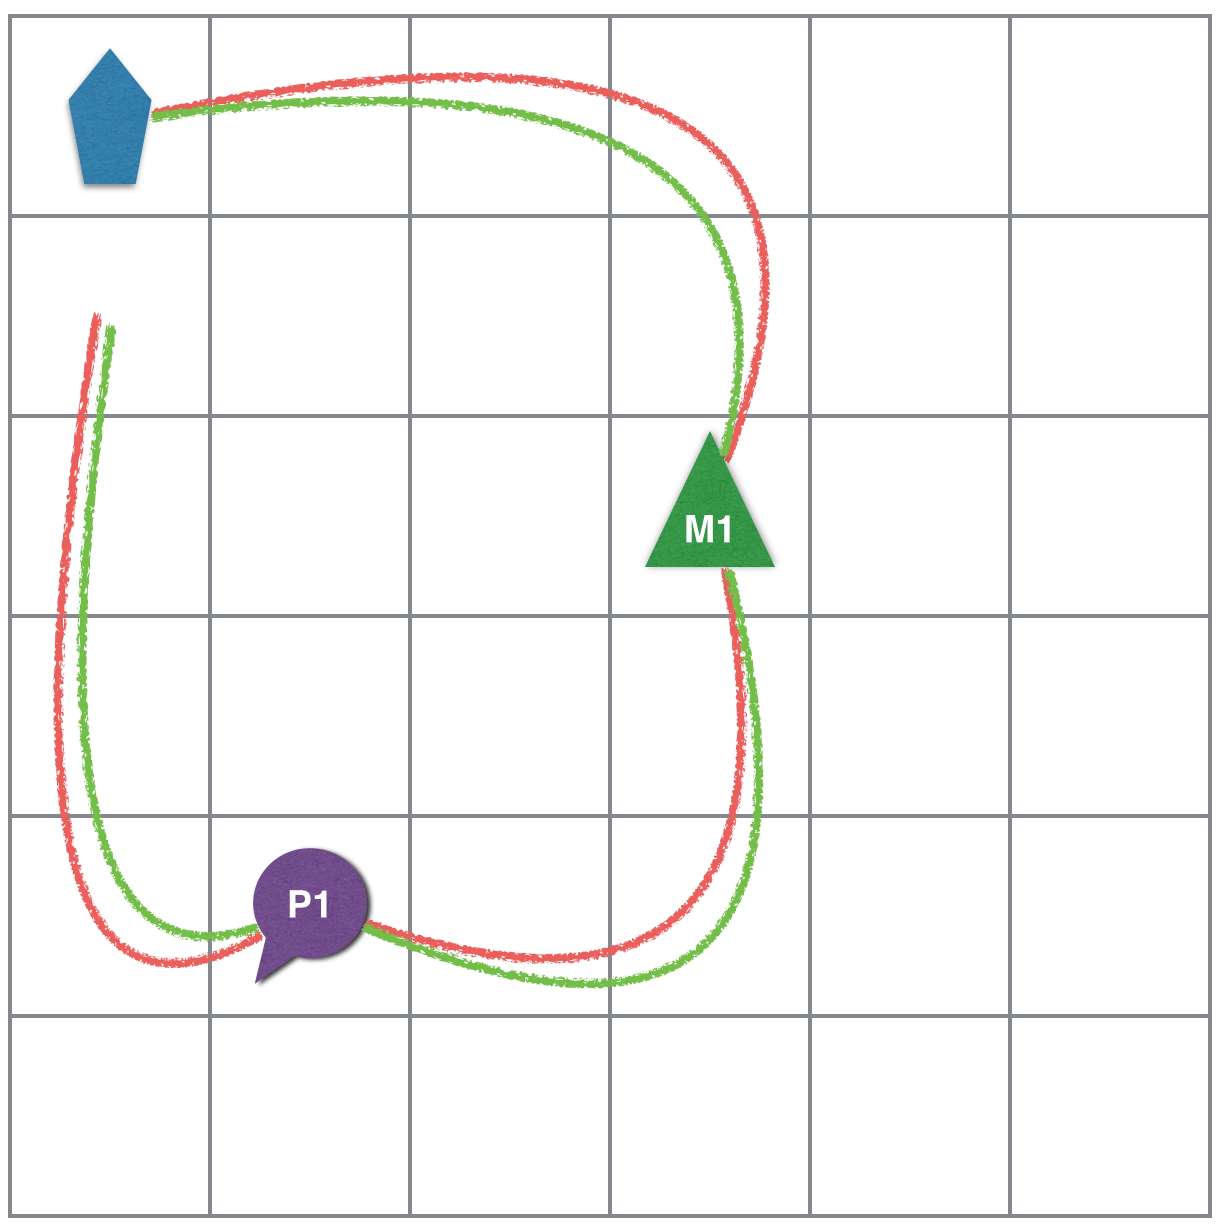
\includegraphics[width=0.5\textwidth]{img/t1}
  \caption{Results for first manually created example}
  \label{fig:t1}
\end{figure}

\begin{figure}[!hbt]
  \centering
  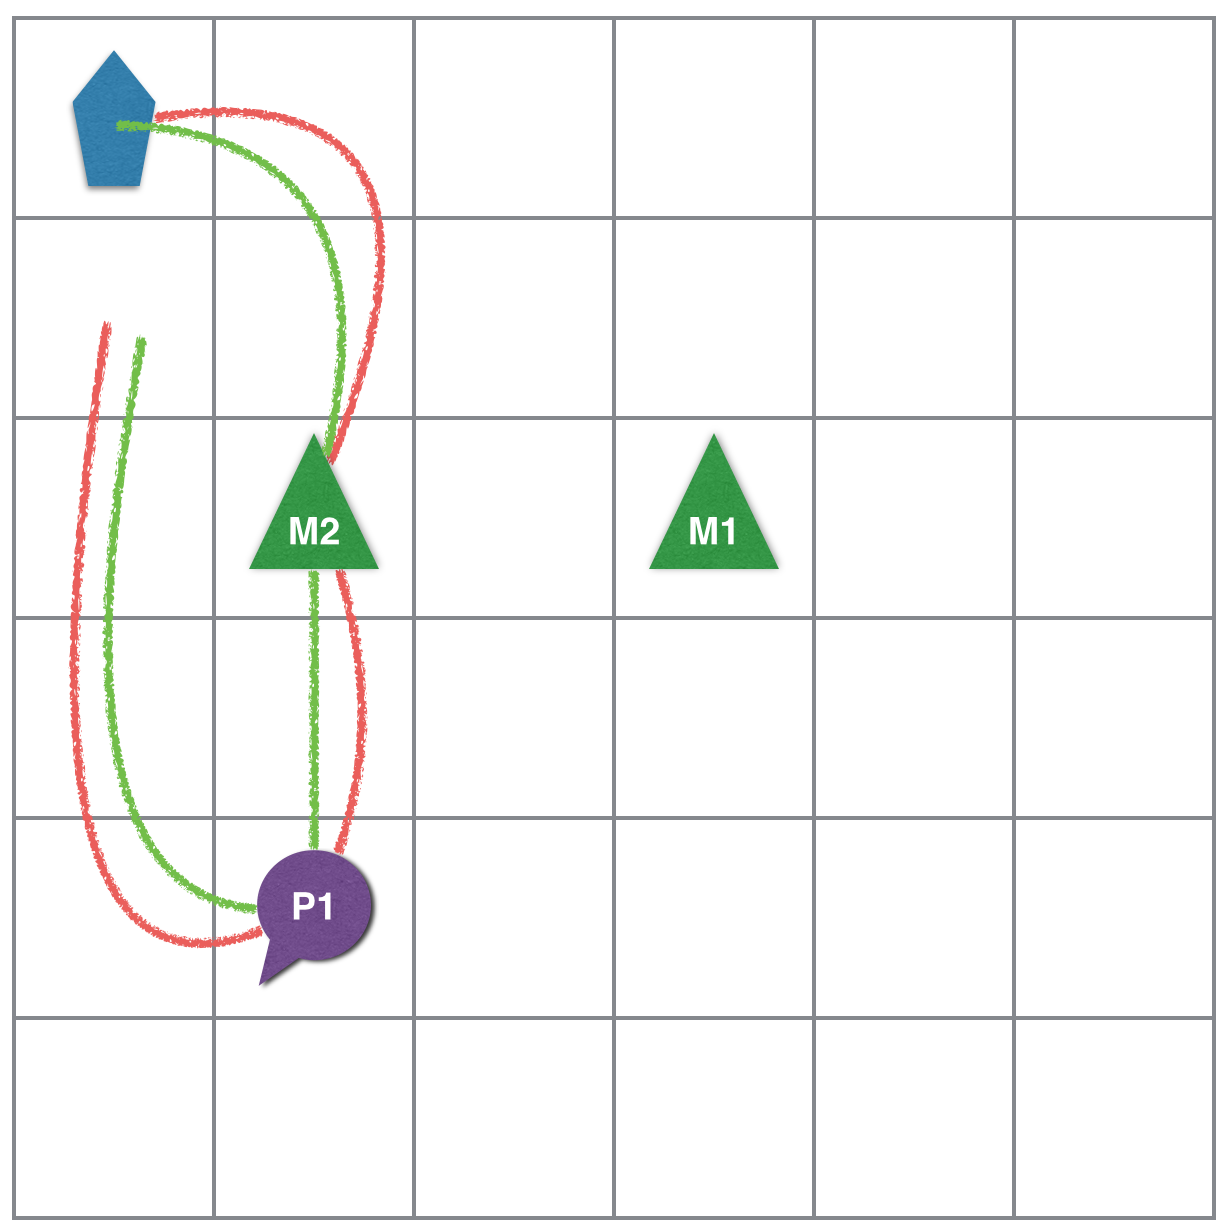
\includegraphics[width=0.5\textwidth]{img/t2}
  \caption{Results for second manually created example}
  \label{fig:t2}
\end{figure}

\begin{figure}[!hbt]
  \centering
  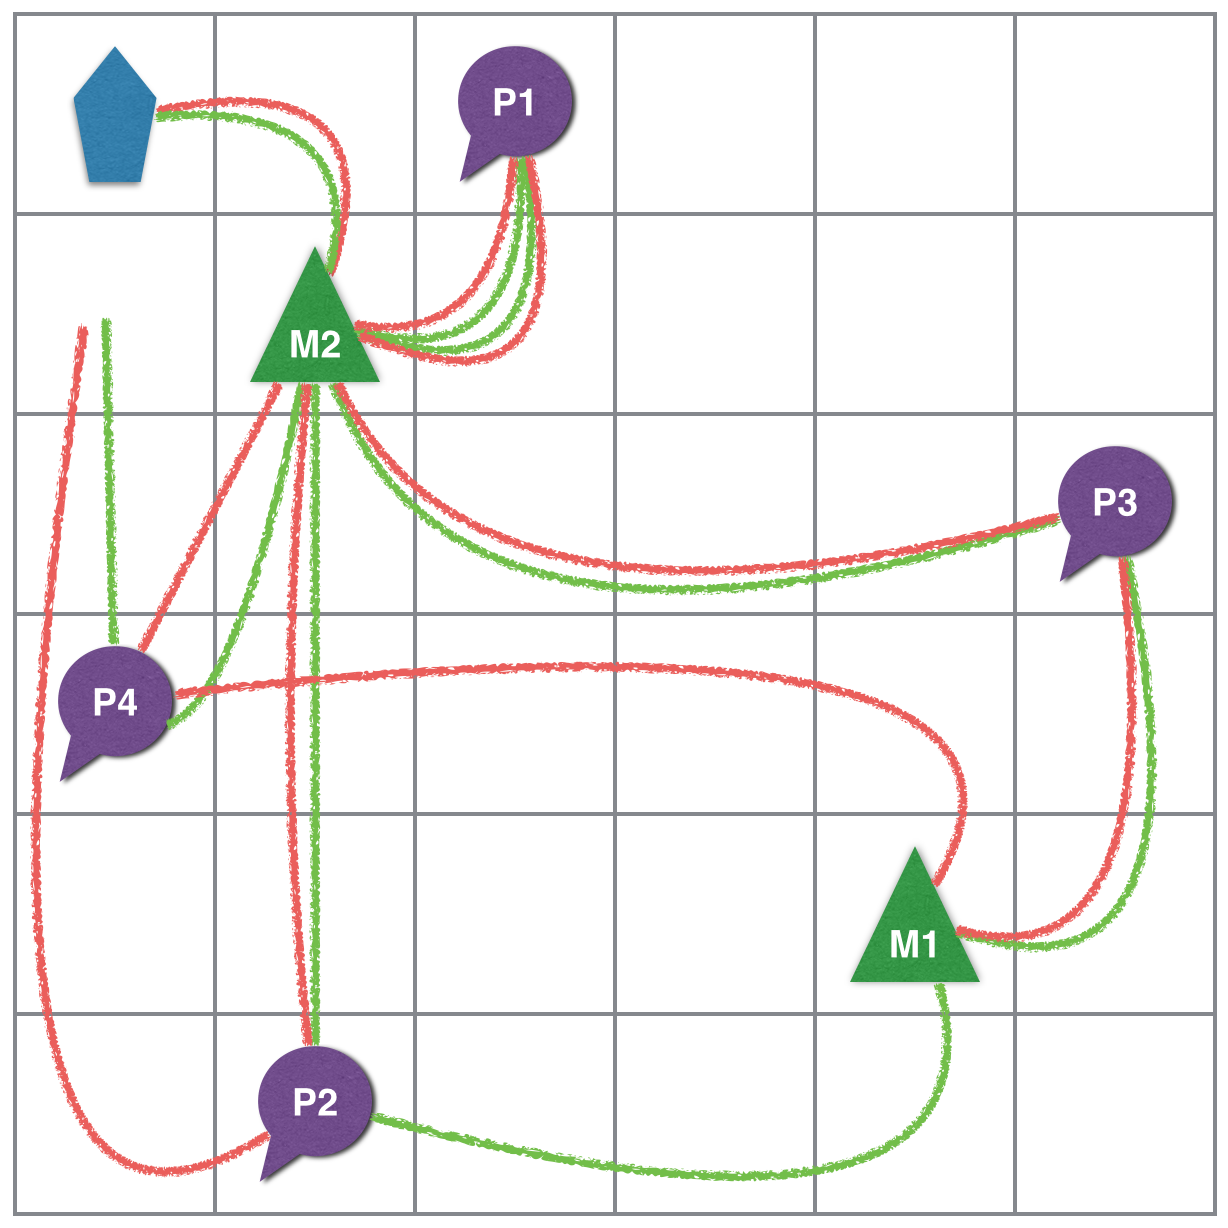
\includegraphics[width=0.5\textwidth]{img/t3}
  \caption{Results for third manually created example}
  \label{fig:t3}
\end{figure}

\subsection{Automatically created worlds}

Figure \ref{fig:abc1} shows the average result (blue dot) and standard deviation (blue bar) of the step error for different heuristics. The step error is defined as the difference between the steps of the optimal solution and the steps that the planner came up with.

NN-TS means, that the NN-heuristic was used to determine the order of petitions. Random means, that a random order of petitions was used. Closest-M means, that the Machine predicate heuristic was used, while First M corresponds to simply picking the first Machine predicate in the list.


\begin{figure}[!hbt]
  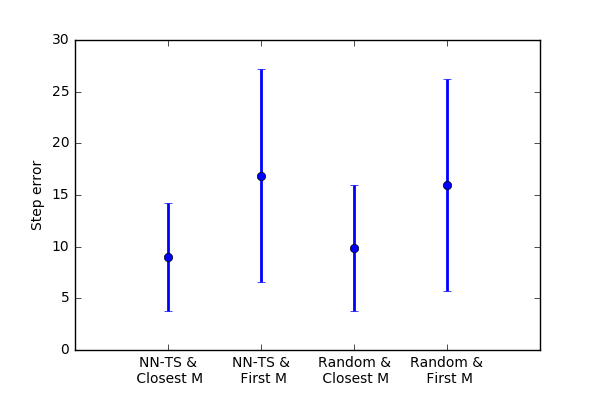
\includegraphics[width=1.1\textwidth]{img/step_error_vs_heuristic}
  \caption{Step Errors for Different Heuristic}
  \label{fig:abc1}
\end{figure}

As we can see in figure \ref{fig:abc1}, using both heuristics yields the best results on average. Not using the NN-heuristics only worsens the results slightly. Deactivating the Machine-heuristic makes the step error increase dramatically - hence it has the highest impact on success.

Figure \ref{fig:abc2} shows how often the different heuristic configuration yielded the smallest step error. Again we can see, that using both heuristics yields the best results with a winner ratio of more than 0.6. The values don't add up to 1.0 because sometimes several strategies had the same result.

\begin{figure}[!hbt]
  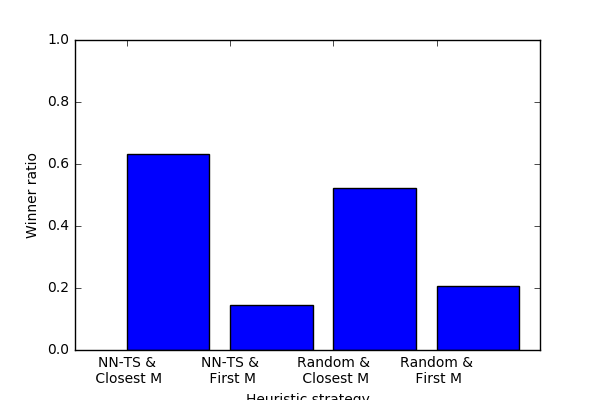
\includegraphics[width=1.1\textwidth]{img/winner_ratio_vs_heuristic}
  \caption{Ratio of Best Solution for Different Heuristic}
  \label{fig:abc2}
\end{figure}

Figure \ref{fig:abc3} shows the relationship between the complexity of the world in terms of numbers of petitions and the average step error. As we can see, for increasing the complexity, using both heuristics yields increasingly better results compared to the other strategies.

\begin{figure}[!hbt]
  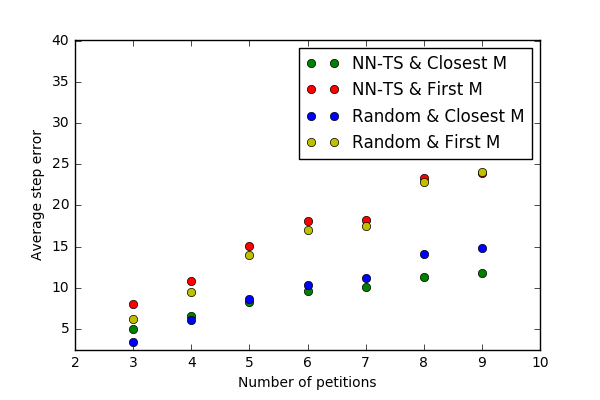
\includegraphics[width=1.1\textwidth]{img/avg_error_vs_petitions}
  \caption{Average Result and Petition Complexity}
  \label{fig:abc3}
\end{figure}

Figure \ref{fig:abc4} shows the relationship between the complexity of the world in terms of numbers of machines and the average step error. There is less correlation between machine complexity and the step error, than we observed with the petition complexity.

\begin{figure}[!hbt]
  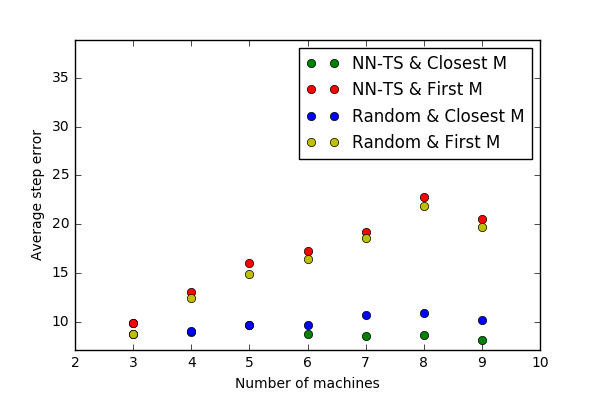
\includegraphics[width=1.1\textwidth]{img/avg_error_vs_machines}
  \caption{Average Result and Machine Complexity}
  \label{fig:abc4}
\end{figure}

